\title{CS534 Implementation Assignment 1:\\Linear Regression, Perceptron}
\author{
        Amit Bawaskar, Michael Lam\\
        EECS, Oregon State University\\
        %\email{}
        %\and
}

\documentclass[12pt]{article}
\usepackage[english]{babel}
\usepackage{graphicx}
\usepackage{subfig}
\usepackage{amsmath}
\usepackage{hyperref}
\hypersetup{
    colorlinks,%
    citecolor=green,%
    filecolor=magenta,%
    linkcolor=red,%
    urlcolor=cyan
}

%\underset{x}{\operatorname{argmax}}
%\underset{x}{\operatorname{argmin}}
\DeclareMathOperator*{\argmin}{arg\,min}
\DeclareMathOperator*{\argmax}{arg\,max}

\begin{document}
\maketitle

\begin{abstract}
In this assignment, we implemented two versions of linear regression and perceptron, and compared their performance.
\end{abstract}

% -------------------------------------------------
\section{Introduction}
We implemented linear regression to solve the regression problem. Two versions were implemented and compared for performance: batch gradient descent and stochastic gradient descent. We also implemented two different versions of perceptron to solve the binary classification problem: batch perceptron and voted perceptron. Voted perceptron provides better behavior for the non-linearly separable case of training data.

\section{Linear Regression}
This section compares the performance of our batch gradient descent and stochastic gradient descent algorithms for linear regression.

\subsection{Batch Gradient Descent}
(Report weight vector for each dataset, SSE for each test set, plot convergence)

\subsection{Stochastic Gradient Descent}
(Report weight vector for each dataset, SSE for each test set, plot convergence)

\section{Perceptron}

Perceptron is a linear Classification model, which is used to create a decision boundary between the various classes of the training data. Whenever a new test data is encountered, we can classify it according to the boundaries generated by the training data. We have implemented two different types of Perceptron algorithms in this assignment, namely Batch Perceptron and Voted Perceptron.

\subsection{Batch Perceptron}

For the given dataset (twogaussian), the Batch Perceptron produced the following results.

Batch Perceptron:

Learned Weights:
   99.0000
  -41.5052
  -34.4167

\begin{figure}[htbp]
  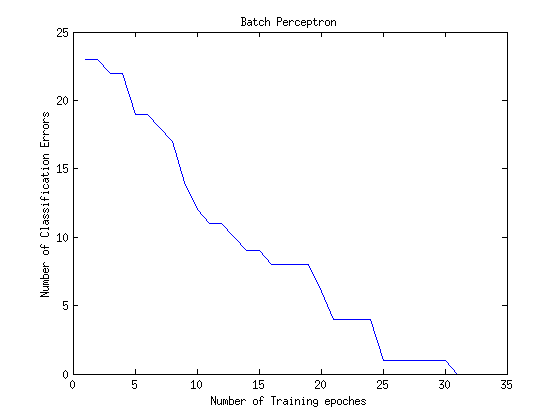
\includegraphics[width=80mm,height=80mm]{img/batch_errors.png}
  \caption{Classification error of Batch Perceptron}
\end{figure}

\begin{figure}[htbp]
  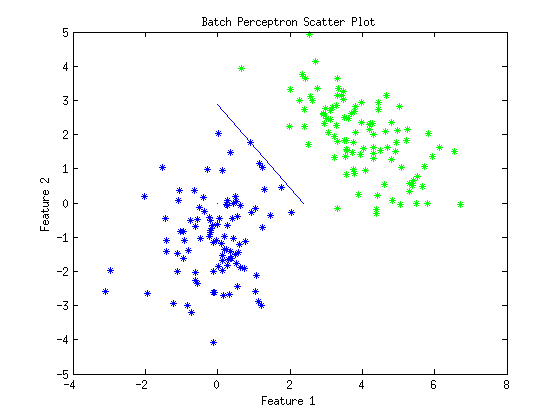
\includegraphics{img/batch_scatterplot.png}
  \caption{Scatter Plot with decision boundary of Batch Perceptron}
\end{figure}
 
(Report plot of classification error on training set, scatter plot of training data)

\subsection{Voted Perceptron}

For the given dataset (iris-twoclass), the Voted Perceptron produced the following results.

Voted Perceptron:

Learned Weights:
\begin{itemize}
  \item 126.0000  
  \item -15.2000
  \item -43.7000
\end{itemize}

Voted Perceptron using averaged weights:

Learned Weights:
  126.0000  
  -15.2000
  -43.7000

The two Learned weights of Voted Perceptron using averaged weights and without using averaged weights are equal, since the result of the stored weight method gets averaged out after every epoch. So the result of averaging all the weight vectors is equal to the result of storing all the weight vectors and calculating the class using that vector.

\begin{figure}[htbp]
  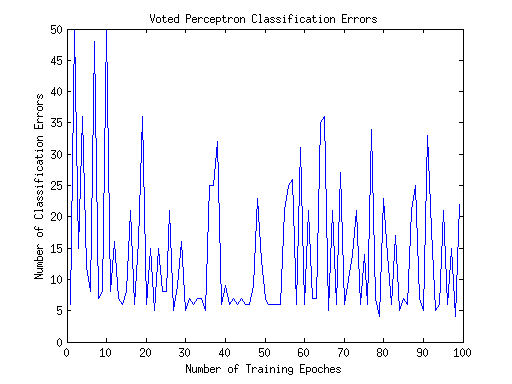
\includegraphics[width=80mm,height=80mm]{img/voted_errors.png}
  \caption{Classification error of Voted Perceptron}
\end{figure}

\begin{figure}[htbp]
  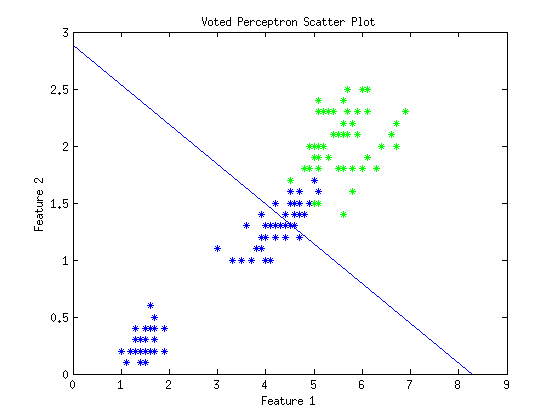
\includegraphics{img/voted_scatterplot.png}
  \caption{Scatter Plot with decision boundary of Voted Perceptron}
\end{figure}

\begin{figure}[htbp]
  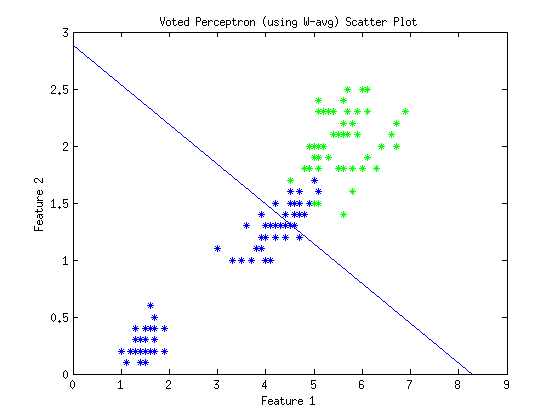
\includegraphics{img/voted_avg_scatterplot.png}
  \caption{Scatter Plot with decision boundary of Voted Perceptron using  averaged weights}
\end{figure}

(Report plot of classification error on training set, visualize decision boundary, report \(w_{avg}\))



\section{Discussion}
Discussion here

\end{document}
This is never printed
